\documentclass{beamer}

% Pacotes utilizados
\usepackage[brazil]{babel}
\usepackage[alf]{abntex2cite}
\usepackage{graphicx,hyperref,url}
\usepackage{uegCCETtheme} % pacote customizado para o curso
\usepackage[T1]{fontenc}
\usepackage[utf8]{inputenc}
\usepackage{ragged2e}
\usepackage{subcaption}
\usepackage{tikz, tkz-euclide, tkz-fct}
\usetikzlibrary{babel}
\usetkzobj{all}

% Título da apresentação [título curto]{título longo}
\title[Cálculo Variacional e o Método de Rayleigh-Ritz]{Uma Introdução ao Cálculo Variacional e ao Método de Rayleigh-Ritz com Aplicações em Python}
%\subtitle{Apenas um subtítulo}
% Autores da apresentação [nome curto]{nome longo}
\author[Eduardo José de Oliveira]{
	Eduardo José de Oliveira\\
	Orientador: Prof. Me. Tiago de Lima Bento Pereira
}
% Nome da instituição [nome curto]{nome longo}
\institute[Universidade Estadual de Goiás]{
	UNIVERSIDADE ESTADUAL DE GOIÁS\\
  	Câmpus Anápolis de Ciências Exatas e Tecnológicas Henrique Santillo \\
  	Matemática
}
% Data [data curta]{data longa}
\date[2019]{2019}
% Observação: geralmente o título\autor\data curto é usado
%             em locais como o rodapé enquanto que o título
%             longo é usado em lugares como a capa, por exemplo.

% declara ambientes matemáticos
\newtheorem{definicao}{Definição}
\newtheorem{lema}{Lema}

\begin{document}

	\begin{frame}[plain]
	  \titlepage
	\end{frame}

	\section{Introdução}
	\begin{frame}
		\frametitle{Introdução}
		
		\justify
		Segundo \citeonline{calcvar} e \citeonline{calcvar_campos}, um dos problemas pertinentes ao Cálculo Variacional é o de minimizar ou maximizar o funcional
		$$
			\int_{x_1}^{x_2} f(x, y, y', y'', \dots, y^{(n)})dx\text{,}
		$$
		isto é, encontrar uma função diferenciável até a ordem $n$, $y=y(x)$, satisfazendo $y(x_1)=y_1$ e $y(x_2)=y_2$, com $x_1$, $x_2$, $y_1$ e $y_2$ dados, tornando a integral um valor mínimo ou máximo.
	\end{frame}
	
	\begin{frame}
		\frametitle{Introdução}
		\justify

		Uma das formas de se encontrar a função $y(x)$ corresponde na determinação da chamada equação de Euler-Lagrange associada ao problema e, então, sua resolução. Além disso, a satisfação das chamadas Condições de Contorno Naturais e Essenciais são necessárias para a correta determinação da função $y(x)$ exata.
		\vspace{10pt}
		\pause
		
		Outra abordagem ao problema consiste na aproximação de $y(x)$ por meio de funções admissíveis.
	\end{frame}
	
	\section{Objetivo}
	\begin{frame}
		\frametitle{Objetivos}
	
		\begin{enumerate}
			\justifying
			\item introduzir, de forma clara e concisa, o Cálculo Variacional por meio do estudo das Equações de Euler-Lagrange para funcionais que dependem de uma única variável, da função e das suas derivadas, até a ordem $n$ desejada;
			
			\item explicar o método de Rayleigh-Ritz, de forma simples e introdutória, desenvolvendo exemplos básicos;
			
			\item apresentar formas de se utilizar a computação para os cálculos do método de Rayleigh-Ritz por meio da linguagem de programação Python.
		\end{enumerate}
	\end{frame}

	\section{Contexto Histórico}
	\makesubtitleframe{Contexto Histórico}

	\begin{frame}
		\frametitle{Máximos e Mínimos}
		\justify
	
		Segundo \citeonline{boyer}, tem-se alguns acontecimentos importantes:
		\begin{itemize}
			\item Pierre de Fermat em 1629.
			\pause
			\begin{itemize}
				\item Comparações entre $f(x)$ e $f(x+E)$ próximo de máximos ou mínimos.
				\pause
				\item Considerar a divisão $\frac{f(x+E)-f(x)}{E}$.
				\pause
				\item Após a divisão, considerar $E=0$.
				\pause
				\item Por último, igualar o resultado a $0$, encontrando as abscissas dos máximos ou mínimos.
			\end{itemize}
			\pause
			\item Cálculo diferencial em 1665 (Isaac Newton) e 1676 (Gottfried Leibniz).
		\end{itemize}
	\end{frame}

	\begin{frame}
		\frametitle{O Problema da Braquistócrona e o Cálculo Variacional}
		\justify
	
		Segundo \citeonline{hist_courant} e \citeonline{hist_still}, o problema da braquistócrona,
		\begin{itemize}
			\item Foi formulado por Johann Bernoulli em 1969 e pode ser apresentado como:
			\begin{block}{Problema da Braquistócrona}
				Sejam $A$ e $B$ dois pontos dados em um plano vertical. O problema da braquistócrona consiste em encontrar a curva que uma partícula M precisa descrever para sair de A e chegar em B no menor tempo possível, somente sob a ação da força da gravidade \cite[p. 3]{calcvar}.
			\end{block}
		\end{itemize}
	\end{frame}

	\begin{frame}
		\frametitle{O Problema da Braquistócrona e o Cálculo Variacional}
		\justify

		Segundo \citeonline{hist_courant} e \citeonline{hist_still},
		\begin{itemize}
			\item A Solução de Jacob Bernoulli (1697) apresenta o aspecto da curva variável.
			\pause
		
			\item Euler e Lagrange.
		\end{itemize}
	\end{frame}
	
	\begin{frame}
		\frametitle{Método de Rayleigh-Ritz}
		\justify
		
		Segundo \citeonline{LEISSA_2005}, 
		\begin{itemize}
			\justifying
			\item O método leva o nome dos pesquisadores Lord Rayleigh e Walter Ritz.
			\pause
			\item Estudado, primeiro, por Lord Rayleigh com problemas de energias potencial e cinética de sistemas.
			\pause
			\item A Generalização foi feita por Walter Ritz.
			\pause
			\item Não se sabe exatamente quando o método passou a se chamar "Método de Rayleigh-Ritz".
		\end{itemize}
	\end{frame}
	
	\begin{frame}
		\frametitle{Aplicação do Método de Rayleigh-Ritz}
		\justify

		Uma das aplicações mais usuais nos trabalhos acadêmicos é o seu uso para a determinação das chamadas frequências naturais.
		\vspace{10pt}
		\pause
		
		As frequências naturais "indicam a taxa de oscilação livre da estrutura, depois de cessada à força que provocou o seu movimento. Em palavras similares, representa o quanto à estrutura vibra quando não há força aplicada sobre ela."\text{ }\cite[p. 1]{Vasquez2015}.
	\end{frame}
	
	\begin{frame}
		\frametitle{Aplicação do Método de Rayleigh-Ritz}
		\justify
		
		Essa aplicação, com as frequências naturais, pode ser verificada nos trabalhos de 
		\begin{itemize}
			\justifying
			\item \citeonline{RRM_Applications} com as vigas consolas.
			\item \citeonline{mrr_beams} com as vigas seguindo os modelos de Timoshenko e de Euler.
			\item \citeonline{GROSSI_2001} com problemas envolvendo placas.
		\end{itemize}
		\vspace{10pt}
		\pause
		
		\citeonline{deep_ritz} estuda a aplicação do Método junto a Inteligência Aritifical, propondo o método chamado de \textit{Deep Ritz Method} para a resolução de problemas variacionais.
	\end{frame}
	
	\encapsulateBackgroundLessFrames{
		\begin{frame}
			\begin{figure}[h]
				\caption{Solução da equação de Poisson em duas dimensões utilizando o \textit{Deep Ritz Method} e o método das diferenças finitas}
				\centering
				\begin{subfigure}{.4\textwidth}
					\centering
					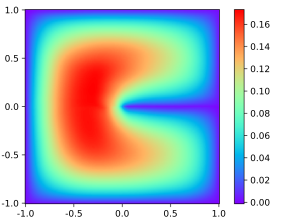
\includegraphics[width=\linewidth]{../figuras/cite/deep_ritz_a.png}
					\caption{Solução pelo \textit{Deep Ritz Method}.}
					\label{fig:deep_ritz_poisson_a}
				\end{subfigure}
				\begin{subfigure}{.4\textwidth}
					\centering
					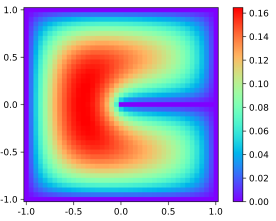
\includegraphics[width=\linewidth]{../figuras/cite/deep_ritz_b.png}
					\caption{Solução pelo método das diferenças finitas.}
					\label{fig:deep_ritz_poisson_b}
				\end{subfigure}
				\label{fig:deep_ritz_poisson}
				\\{\small Fonte: \citeonline[p. 5]{deep_ritz}.}
			\end{figure}
		\end{frame}
	}
	
	\begin{frame}
		\frametitle{Linguagem Python}
		\justify
		
		\begin{itemize}
			\justifying
			\item Criada por Guido van Rossum por volta de 1990.
			\pause
			\item Desenvolvimento \textit{open-source}.
			\pause
			\item Atualmente há cerca de 1000 colaboradores no GitHub.
			\pause
			\item Diversas bibliotecas de rotinas como, por exemplo, o ecossistema SciPy:
				\begin{itemize}
					\item NumPy
					\item SciPy
					\item MatplotLib
					\item SymPy\\
					...
				\end{itemize}
		\end{itemize}
	\end{frame}

	\section{Cálculo Variacional}
	\makesubtitleframe{Cálculo Variacional}
	
	\begin{frame}
		\frametitle{Cálculo Variacional}
		\justify
		
		{\color{red}Falar do Cálculo Variacional.}
	\end{frame}

	%\begin{frame}
	%	\frametitle{Relembrando o problema}
	%	\justify
	%
	%	Deseja-se, no Cálculo Variacional, encontrar uma função diferenciável até segunda ordem $y=y(x)$ satisfazendo $y(x_1)=y_1$ e $y(x_2)=y_2$, com $x_1$, $x_2$, $y_1$ e $y_2$ dados, e $f$ uma função duas vezes diferenciável, minimizando ou maximizando a integral
	%	\begin{equation}
	%		\int_{x_1}^{x_2} f(x,y,y')dx\text{.}
	%		\label{eqn:def_calcvar}
	%	\end{equation}
	%\end{frame}

	%\begin{frame}
	%	\frametitle{Funções Aproximadoras}
	%	\begin{definicao}
	%		\justify
	%		Uma família de funções aproximadoras é definida como
	%		$$Y(x)=y(x)+\varepsilon \eta (x)\text{,}$$
	%		onde a função $\eta (x)$ é uma função diferenciável arbitrária para a qual $\eta (x_1)=\eta (x_2)=0$. O número $\varepsilon$ é o parâmetro da família. Sua derivada pode ser escrita como
	%		$$Y'(x)=y'(x)+\varepsilon \eta '(x)\text{.}$$
	%	\end{definicao}
	%\end{frame}

	%\encapsulateBackgroundLessFrames
	%{
	%	\begin{frame}
	%		\begin{figure}
	%			\caption{Representação gráfica das funções aproximadoras.}
	%			\begin{center}
	%				\resizebox{0.5\textwidth}{0.5\textwidth}{
	%					\begin{tikzpicture}
	\tkzInit[xmin=-1, xmax=6, ymin=-1, ymax=6]
	% draw axis without ticks
	\tkzDrawX[noticks]
	\tkzDrawY[noticks]
	
	% define extrems on y(x) curve
	\tkzDefPoint[](2.5, 2.0){A}
	\tkzDefPoint[](4.6, 3.76){B}		
	% define helper points
	\tkzDefPoint[](2.5, 0.0){C}
	\tkzDefPoint[](4.6, 0.0){D}
	\tkzDefPoint[](0.0, 2.0){E}
	\tkzDefPoint[](0.0, 3.76){F}
	% helper points to put labels
	\tkzDefPoint[](3.4, 3.2){G}
	\tkzDefPoint[](2.6, 1.7){H}
	\tkzDefPoint[](3.7, 4.2){I}
	\tkzDefPoint[](3.2, 0.4){J}
	
	% draw extrem points on y(x) curve
	\tkzDrawPoint[fill=black, size=7](A)
	\tkzDrawPoint[fill=black, size=7](B)
		
	% y(x)
	\tkzFct[domain=2.5:4.6,samples=1000, line width=2pt]{-exp(-x+3.2)+4}
	% eta(x)
	\tkzFct[domain=2.5:4.6,samples=1000]{-0.18*x*x+1.29*x-2.09}
	% y(x) + 2*eta(x)
	\tkzFct[domain=2.5:4.6,samples=1000,dashed]{-exp(-x+3.2)+4+2*(-0.18*x*x+1.29*x-2.09)}
	% y(x) - 4*eta(x)
	\tkzFct[domain=2.5:4.6,samples=1000,dashed]{-exp(-x+3.2)+4-4*(-0.18*x*x+1.29*x-2.09)}
		
	% draw dotted segments (x_1, y_1), (x_2, y_2)
	\tkzDrawSegment[dotted](A,C)
	\tkzDrawSegment[dotted](B,D)
	\tkzDrawSegment[dotted](A,E)
	\tkzDrawSegment[dotted](B,F)
		
	% x_1, x_2, y_1, y_2 labels
	\tkzLabelPoint[below](C){$x_1$}
	\tkzLabelPoint[below](D){$x_2$}
	\tkzLabelPoint[left](E){$y_1$}
	\tkzLabelPoint[left](F){$y_2$}
	
	\tkzLabelPoint[right](G){$y(x)$}
	\tkzLabelPoint[right](H){$Y_2(x)=y(x)+\varepsilon _2 \eta(x)$}
	\tkzLabelPoint[right](I){$Y_1(x)=y(x)+\varepsilon _1 \eta(x)$}
	\tkzLabelPoint[right](J){$\eta(x)$}
\end{tikzpicture}
	%				}\\
	%				{\small Fonte: Elaborada pelo autor, 2019.}
	%			\end{center}
	%			\label{fig:func_approx}
	%		\end{figure}
	%	\end{frame}
	%}
	
	%\begin{frame}
	%	\frametitle{Reescrevendo o Problema}
	%	\justify
	%
	%	Pode-se reescrever a integral \eqref{eqn:def_calcvar} utilizando as funções aproximadoras, dependendo de $\varepsilon$, então
	%	\begin{equation}
	%		\label{eqn:int_funcional_approx}
	%		I(\varepsilon)=\int_{x_1}^{x_2}f(x, Y, Y')dx\text{.}
	%	\end{equation}
	%
	%	Para encontrar a função $y(x)$ que maximiza ou minimiza a integral escrita com as funções aproximadoras \eqref{eqn:int_funcional_approx}, deve-se fazer
	%	$$I'(\varepsilon)=0\text{,}$$
	%	e, considerando que quando $\varepsilon=0$, as integrais \eqref{eqn:def_calcvar} e \eqref{eqn:int_funcional_approx} fornecem os mesmos maximos e mínimos, é necessário que
	%	$$I'(0)=0\text{.}$$
	%\end{frame}

	%\begin{frame}
	%	\justify
	%
	%	Utilizando a Regra de Leibniz, pode-se escrever a derivada de $I(\varepsilon)$ como
	%	$$I'(\varepsilon)=\int_{x_1}^{x_2} \frac{\partial f}{\partial \varepsilon} (x, Y, Y') dx \text{,}$$
	%	\pause
	%	donde, aplicando a regra da cadeia, obtêm-se
	%	$$I'(\varepsilon)=\int_{x_1}^{x_2}\left ( \frac{\partial f}{\partial x}\frac{\partial x}{\partial \varepsilon} + \frac{\partial f}{\partial Y} \frac{\partial Y}{\partial \varepsilon} + \frac{\partial f}{\partial Y'} \frac{\partial Y'}{\partial \varepsilon} \right )dx\text{.}$$
	%	\pause
	%
	%	O primeiro termo do integrando é nulo, pois $x$ independe de $\varepsilon$, então
	%	$$
	%		I'(\varepsilon)=\int_{x_1}^{x_2}\left ( \frac{\partial f}{\partial Y}\frac{\partial Y}{\partial \varepsilon} + \frac{\partial f}{\partial Y'}\frac{\partial Y'}{\partial \varepsilon} \right ) dx \text{.}
	%	$$
	%\end{frame}

	%\begin{frame}
	%	\justify
	%
	%	Derivando a função aproximadora $Y(x)=y(x)+\varepsilon \eta(x)$ em relação a $\varepsilon$, conclui-se que
	%	$$\frac{\partial Y}{\partial \varepsilon}=\eta\text{.}$$
	%	\pause
	%
	%	De modo análogo, ao derivar $Y'(x)=y'(x)+\varepsilon \eta '(x)$ em relação a $\varepsilon$, obtêm-se que
	%	$$\frac{\partial Y'}{\partial \varepsilon}=\eta '\text{.}$$
	%\end{frame}

	%\begin{frame}
	%	\justify
	%
	%	Substituindo $\frac{\partial Y}{\partial \varepsilon}=\eta$ e $\frac{\partial Y'}{\partial \varepsilon}=\eta'$ em $I'(\varepsilon)$,
	%	$$
	%		I'(\varepsilon)=\int_{x_1}^{x_2}\left ( \frac{\partial f}{\partial Y}\frac{\partial Y}{\partial \varepsilon} + \frac{\partial f}{\partial Y'}\frac{\partial Y'}{\partial \varepsilon} \right ) dx
	%	$$
	%	\pause
	%	$$
	%		I'(\varepsilon)=\int_{x_1}^{x_2}\left ( 
	%			\frac{\partial f}{\partial Y} \eta +
	%			\frac{\partial f}{\partial Y'} \eta '
	%		\right )dx \text{.}
	%	$$
	%\end{frame}

	%\begin{frame}
	%	\justify
	%
	%	Calculando $I'(0)$, ou seja, quando $\varepsilon=0$, é possível trocar $Y$ e $Y'$ por $y$ e $y'$, respectivamente, então,
	%	$$
	%		I'(0)=\int_{x_1}^{x_2}\left (
	%			\frac{\partial f}{\partial y} \eta +
	%			\frac{\partial f}{\partial y'} \eta '
	%		\right )dx
	%	$$
	%	\pause
	%	$$
	%		I'(0)=
	%			\int_{x_1}^{x_2} \frac{\partial f}{\partial y}\eta dx
	%			+
	%			\int_{x_1}^{x_2} \frac{\partial f}{\partial y'}\eta' dx \text{.}
	%	$$
	%	\pause
	%
	%	Integrando o segundo membro por partes, tem-se
	%	$$
	%	I'(0)=
	%		\int_{x_1}^{x_2} \frac{\partial f}{\partial y}\eta dx
	%		-
	%		\int_{x_1}^{x_2} \frac{d}{dx} \left ( \frac{\partial f}{\partial y'} \right ) \eta dx
	%	$$
	%\end{frame}
	
	%\begin{frame}
	%	\justify
	%
	%	Organizando $I'(0)$, tem-se
	%	$$
	%		I'(0)=\int_{x_1}^{x_2}\left (
	%			\frac{\partial f}{\partial y} -
	%			\frac{d}{dx}
	%			\left (
	%				\frac{\partial f}{\partial y'}
	%			\right )
	%		\right )\eta dx
	%		\text{.}
	%	$$
	%	\pause
	%	
	%	Devido a condição necessária, $I'(0)=0$, escrevemos
	%	$$
	%		I'(0)=\int_{x_1}^{x_2}\left (
	%			\frac{\partial f}{\partial y} -
	%			\frac{d}{dx}
	%			\left (
	%				\frac{\partial f}{\partial y'}
	%			\right )
	%		\right )\eta dx = 0
	%		\text{.}
	%	$$
	%\end{frame}

	%\begin{frame}
	%	\justify
	%	Para concluirmos a dedução do resultado é necessário o uso do seguinte lema:
	%
	%	\begin{lema}
	%		\justify
	%		Sejam $x_1 < x_2$ fixos e $G(x)$ uma função contínua particular para $x_1 \leqslant x \leqslant x_2$. Se $$\int_{x_1}^{x_2} \eta (x) G(x) dx = 0$$ para cada função diferenciável $\eta (x)$ tal que $\eta (x_1)=\eta (x_2)=0$, concluímos que $G(x)=0$, para todo $x$ de modo que $x_1 \leqslant x \leqslant x_2$.
	%	\end{lema}	
	%
	%\end{frame}

	%\begin{frame}
	%	\frametitle{Equação de Euler-Lagrange}
	%	\justify
	%
	%	Pelo Lema anterior, conlui-se que
	%	$$
	%		\frac{\partial f}{\partial y} - \frac{d}{dx} \left ( \frac{\partial f}{\partial y'} \right )=0 \text{.}
	%	$$
	%	\pause
	%
	%	A equação acima é chamada de \textbf{Equação de Euler-Lagrange}, sendo uma condição necessária para minimizar ou maximizar a integral
	%	$$
	%		\int_{x_1}^{x_2} f(x, y, y')dx \text{.}
	%	$$
	%\end{frame}
	
	%
	% Método de Rayleigh-Ritz
	%
	
	\section{Método de Rayleigh-Ritz}
	\makesubtitleframe{Método de Rayleigh-Ritz}
	
	\begin{frame}
		\frametitle{Método de Rayleigh-Ritz}
		\justify
		
		A determinação da função exata $y(x)$ nem sempre é fácil ou possível. O método de Rayleigh-Ritz propõe que a função $y(x)$ seja substituida por uma função aproximada $v(x)$.
		\vspace{10pt}
		\pause
		
		Considere o funcional
		$$
			I = \int_{x_1}^{x_2} f(x, y, y', y'', \dots, y^{(n)})dx\text{,}
		$$
		com as condições de contorno $y(x_1)=y(x_2)=0$.
	\end{frame}
	
	\begin{frame}
		\frametitle{Método de Rayleigh-Ritz}
		\justify
		
		Seja
		$$
			y(x) \approx v(x)=\sum_{i=1}^n a_i \phi_i(x)
			\text{.}
		$$
		\vspace{10pt}
		\pause
		
		Substituindo $y$ por $v$ no funcional, tem-se $I=I(a_1, a_2, \dots, a_n)$.
		\vspace{10pt}
		\pause
		
		A condição de máximo ou mínimo para $I$ é, agora, que
		$$
			\frac{\partial I}{\partial a_i} = 0
			\text{,}
		$$
		onde $i=1,2,\dots,n$.
	\end{frame}
	
	% Exemplo
	\begin{frame}
		\frametitle{Método de Rayleigh-Ritz}
		\justify
		
		\begin{itemize}
			\begin{block}{Exemplo}
				\justify
				Uma viga prismática possui o funcional de energia potencial total associado
				$$
					\Pi = 
					\frac{1}{2} \int_0^l EI \left [
						\frac{d^2v}{dx^2}
					\right ]^2 dx
					-
					\int_0^l qvdx
					\text{,}
				$$
				onde $E$ é o módulo de Young do material e I é o momento de inércia da seção transversal da viga em relação ao eixo baricêntrico.
			\end{block}
		\end{itemize}
	\end{frame}
	
	% Figura do Exemplo
	\encapsulateBackgroundLessFrames
	{
		\begin{frame}
			\begin{figure}[h]
				\caption{Viga prismática.}
				\centering
				\begin{tikzpicture}
					\tkzInit[xmin=-0, xmax=6, ymin=-0.6, ymax=2]
					% draw axis without ticks
					\tkzDrawX[label=$x$, noticks, loosely dashed]
					\tkzDrawY[label=$v(x)$, noticks]
					
					% rectangle
					\tkzDefPoints{
						0/0.6/V_1,
						5/0.6/V_2,
						5/-0.6/V_3,
						0/-0.6/V_4}
					% complete x axis without dashed line
					\tkzDefPoints{
						5/0/A_1,
						6.35/0/A_2}
					% left base triangle
					\tkzDefPoints{
						0/-0.6/T1_1, 
						-0.25/-1.1/T1_2, 
						0.25/-1.1/T1_3}
					% right base triangle
					\tkzDefPoints{
						5/-0.6/T2_1, 
						4.75/-1.1/T2_2,
						5.25/-1.1/T2_3}
					% line on base of right triangle
					\tkzDefPoints{
						4.75/-1.2/T2_B1,
						5.25/-1.2/T2_B2}
					% length marker in bottom
					\tkzDefPoints{
						0/-1.5/L_1,
						0/-2/L_2,
						5/-1.5/L_3,
						5/-2/L_4,
						0/-1.75/LS_1,
						5/-1.75/LS_2}
					
					\tkzDrawSegment[color=black, line width=0.5mm](A_1, A_2)
					
					\tkzDrawPolygon[draw=black](T1_1, T1_2, T1_3)
					\tkzDrawPolygon[draw=black](T2_1, T2_2, T2_3)
					\tkzDrawSegment[color=black](T2_B1, T2_B2)
					\tkzDrawPolygon[draw=black](V_1, V_2, V_3, V_4)
					% q arrows
					\foreach \i in {1,...,25}{
						\tkzDefPoint(0.2*\i,1.3){A_\i}
						\tkzDefPoint(0.2*\i,0.7){B_\i}
						\draw[line width=0.6pt, black,-stealth] (A_\i) -- (B_\i);
					}
					% q text
					\node at (2.5,1.7) {$q$};
					% length marker in bottom
					\tkzDrawSegment[color=black](L_1, L_2)
					\tkzDrawSegment[color=black](L_3, L_4)
					\tkzDrawSegment[color=black](LS_1, LS_2)
					\node at (2.5,-2) {$l$};
				\end{tikzpicture}
				\\{\small Fonte: \citeonline[p. 25]{mefassan}.}
			\end{figure}
		\end{frame}
	}
	
	% Resolução do Exemplo
	\begin{frame}
		\frametitle{Método de Rayleigh-Ritz}
		\justify
		
		Seja $v_1(x)=a_0 + a_1 x + a_2 x^2$. \pause Das condições de contorno
		$$
			v_1(0)=0\Longrightarrow a_0 = 0\text{,}
		$$
		\pause
		$$
			v_1(l)=0\Longrightarrow a_1 = -a_2l\text{.}
		$$
		\pause
		Logo, $v_1(x)=a_2(x^2-lx)$, \pause $v_1'(x)=a_2(2x-l)$ \pause e $v_1''(x)=2a_2$.
	\end{frame}
	
	\begin{frame}
		\frametitle{Método de Rayleigh-Ritz}
		\justify
		
		Substituindo $v$ por $v_1$ em $\Pi$,
		$$
			\Pi =
			\frac{1}{2}
			\int_0^l 4 EI a_2 ^2 dx
			-
			\int_0^l q a_2 (x^2-lx) dx
			\text{.}
		$$
		\pause
		
		Da condição de estacionariedade, $\dfrac{\partial \Pi}{\partial a_2}=0$,
		$$
			a_2 = -\frac{ql^2}{24EI}
			\text{.}
		$$
		\pause
		E, como $a_1=-a_2l$,
		$$
			a_1 = \frac{ql^3}{24EI}
			\text{.}
		$$
	\end{frame}
	
	\begin{frame}
		\frametitle{Método de Rayleigh-Ritz}
		\justify
		
		Assim, 
		$$
			v_1(x)=\dfrac{ql^3}{24EI}x - \dfrac{ql^2}{24EI}x^2
			\text{.}
		$$
		\pause
		
		Calculando o valor de máxima deflexão,
		$$
			v_1\left ( \frac{l}{2} \right )
			= \frac{ql^4}{96EI}
			\text{.}
		$$
		\pause
		
		O valor de máxima deflexão para $v_1(x)$ é menor que o valor exato,
		$$
			v\left ( \frac{l}{2} \right )
			= \frac{5ql^4}{384EI}
			\text{.}
		$$
	\end{frame}
	
	\begin{frame}
		\frametitle{Método de Rayleigh-Ritz}
		\justify
		
		Seja $v_2(x)=a_0 + a_1 x + a_2 x^2 + a_3 x^3$. \pause Das condições de contorno
		$$
			v_2(0)=0\Longrightarrow a_0 = 0\text{,}
		$$
		\pause
		$$
			v_2(l)=0\Longrightarrow a_1 = -a_2l - a_3l^2\text{.}
		$$
		\pause
		Logo, 
		$$v_2(x)=a_2(x^2-lx)+a_3(x^3-l^2x)\text{,}$$
		\pause 
		$$v_2'(x)=a_2(2x-l)+a_3(3x^2-l^2)\text{,}$$
		\pause
		$$v_2''(x)=2a_2 + 6a_3x\text{.}$$
	\end{frame}
	
	\begin{frame}
		\frametitle{Método de Rayleigh-Ritz}
		\justify
		
		Substituindo $v$ por $v_2$ em $\Pi$,
		$$
			\Pi=
			\frac{1}{2}
			\int_0^l
				\left (
					EI(2a_2+6a_3x)^2
				\right ) dx
			-
			\int_0^l
				q
				\left (
					a_2(x^2-lx)
					+
					a_3(x^3-l^2x)
				\right ) dx
			\text{.}
		$$
		\pause
		Da condição de estacionariedade, tem-se o sistema
		$$
			\begin{cases}
				\dfrac{\partial \Pi}{\partial a_2}=0\\[10pt]
				\dfrac{\partial \Pi}{\partial a_3}=0
			\end{cases}
			\text{.}
		$$
	\end{frame}
	
	\begin{frame}
		\frametitle{Método de Rayleigh-Ritz}
		\justify
		
		$$
			\begin{cases}
				2a_2+3a_3l=\dfrac{-ql^2}{12EI}\\[10pt]
				2a_2+4a_3l=\dfrac{-ql^2}{12EI}
			\end{cases}
			\text{.}
		$$
		\pause
		Resolvendo o sistema,
		$$
			a_3=0
			\text{,}
		$$
		\pause
		$$
			a_2=-\frac{ql^2}{24EI}
			\text{.}
		$$
	\end{frame}
	
	\begin{frame}
		\frametitle{Método de Rayleigh-Ritz}
		\justify
		
		Seja $v_3(x)=a_0 + a_1 x + a_2 x^2 + a_3 x^3 + a_4 x^4$. \pause Das condições de contorno
		$$
			v_3(0)=0\Longrightarrow a_0 = 0\text{,}
		$$
		\pause
		$$
			v_3(l)=0\Longrightarrow a_1 = -a_2l - a_3l^2 - a_4l^3\text{.}
		$$
		\pause
		Logo, 
		$$v_3(x)=a_2(x^2-lx)+a_3(x^3-l^2x) + a_4(x^4-l^3x)\text{,}$$
		\pause 
		$$v_3'(x)=a_2(2x-l)+a_3(3x^2-l^2)+a_4(4x^3-l^3)\text{,}$$
		\pause
		$$v_3''(x)=2a_2 + 6a_3x + 12a_4x^2\text{.}$$
	\end{frame}
	
	\begin{frame}
		\frametitle{Método de Rayleigh-Ritz}
		\justify
		
		Substituindo $v$ por $v_3$ em $\Pi$,
		$$
			\Pi = \frac{1}{2} \int_0^l \left [
				EI(2a_2+6a_3x+12a_4x^2)^2
			\right ] dx
			-
		$$
		$$
			-
			\int_0^l q \left [
				a_2(x^2 - lx)
				+
				a_3(x^3 - l^2x)
				+
				a_4(x^4 - l^3x)
			\right ] dx
			\text{.}
		$$
	\end{frame}
	
	\begin{frame}
		\frametitle{Método de Rayleigh-Ritz}
		\justify
		Da condição de estacionariedade, tem-se o sistema
		$$
			\begin{cases}
				\dfrac{\partial \Pi}{\partial a_2}=0\\[10pt]
				\dfrac{\partial \Pi}{\partial a_3}=0\\[10pt]
				\dfrac{\partial \Pi}{\partial a_4}=0
			\end{cases}
			\text{.}
		$$
	\end{frame}
	
	\begin{frame}
		\frametitle{Método de Rayleigh-Ritz}
		\justify
		
		$$
			\begin{cases}
				2a_2 + 3a_3l + 4a_4l^2 = -\dfrac{ql^2}{12EI}\\[10pt]
				a_2 + 2a_3 l + 3a_4 l^2 = - \dfrac{ql^2}{24EI}\\[10pt]
				8a_2 + 18a_3 l + \dfrac{144}{5} a_4 l^2 =-\dfrac{3ql^2}{10EI}
			\end{cases}
		$$
		\pause
		Resolvendo o sistema, tem-se
		$$
			a_2 = 0
			\text{,}
		$$
		\pause
		$$
			a_3 = -\frac{ql}{12EI}
			\text{,}
		$$
	\end{frame}
	
	\begin{frame}
		\frametitle{Método de Rayleigh-Ritz}
		\justify
	
		$$
			a_4 = \frac{q}{24EI}
			\text{.}
		$$
		\pause
		Como $a_1=-a_2l - a_3l^2-a_4l^3$,
		$$
			a_1 = \frac{ql^3}{24EI}
			\text{.}
		$$
		\pause
		A função $v_3$ é
		$$
			v_3(x)=
			\frac{ql^3}{24EI} x
			-
			\frac{ql}{12EI} x^3
			+
			\frac{q}{24EI} x^4
			\text{.}
		$$
	\end{frame}
	
	\begin{frame}
		\frametitle{Método de Rayleigh-Ritz}
		\justify
		
		O valor de máxima deflexão é identico,
		$$
			v_3\left ( \frac{l}{2} \right )
			=
			v\left ( \frac{l}{2} \right )
			= \frac{5ql^4}{384EI}
			\text{.}
		$$
		\pause
		
		A função $v_3(x)$ é, de fato, a função exata $v(x)$.
	\end{frame}
	
	%
	% Uso de funções triangulares
	%
	\makesubtitleframe{O Uso de Funções Triangulares no Método de Rayleigh-Ritz}
	
	\begin{frame}
		\frametitle{Funções Triangulares}
		
		{\color{red}Explicar o uso das funções triangulares.}
	\end{frame}
	
	\section{Método de Rayleigh-Ritz e a Linguagem Python}
	\makesubtitleframe{Método de Rayleigh-Ritz e a Linguagem Python}
	 
	\begin{frame}
		\frametitle{Método de Rayleigh-Ritz e a Linguagem Python}
		
		{\color{red}Explicar sobre o uso da Linguagem Python.}
	\end{frame}

	\section{Referências}
	\begin{frame}[allowframebreaks]
		\frametitle{Referências}
		\bibliography{../references}
	\end{frame}

\end{document}